%% ============================================================
%% Biên dịch bằng XeLaTeX (Overleaf: Menu > Compiler > XeLaTeX)
%% Các hình kết quả cũ được lưu trong legacy/results/.
%% Biên dịch từ thư mục gốc dự án để giữ nguyên đường dẫn tương đối.
%% ============================================================
\documentclass[12pt,a4paper]{report}
\usepackage{fontspec}
\usepackage{polyglossia}
\setdefaultlanguage{vietnamese}
\IfFontExistsTF{TeX Gyre Termes}{\setmainfont{TeX Gyre Termes}}{\setmainfont{Times New Roman}}
\IfFontExistsTF{TeX Gyre Heros}{\setsansfont{TeX Gyre Heros}}{\setsansfont{Arial}}
\IfFontExistsTF{Latin Modern Mono}{\setmonofont{Latin Modern Mono}}{\setmonofont{Courier New}}
\usepackage[a4paper,top=2.5cm,bottom=2.5cm,left=3cm,right=2cm]{geometry}
\usepackage{setspace}\setstretch{1.12}\usepackage{indentfirst}
\setlength{\parindent}{1.0cm}\setlength{\parskip}{0pt}
\usepackage{microtype,graphicx,float,booktabs,tabularx,array,amsmath,amssymb,caption,chngcntr}
\counterwithout{figure}{chapter}\counterwithout{table}{chapter}
\usepackage{tikz}\usetikzlibrary{arrows.meta,positioning,shapes.geometric}
\usepackage[numbers,sort&compress]{natbib}
\usepackage{hyperref}
\hypersetup{colorlinks=true,linkcolor=black,citecolor=black,urlcolor=blue,
 pdftitle={Ứng dụng học liên kết kết hợp quyền riêng tư vi phân để phân loại u não từ ảnh MRI trên dữ liệu phân tán}}
\usepackage{titlesec}
\titleclass{\chapter}{straight}
\titleformat{\chapter}[hang]{\normalfont\bfseries\LARGE}{\thechapter}{0.8em}{}
\titlespacing*{\chapter}{0pt}{18pt}{10pt}
\titleformat{\section}{\normalfont\bfseries\Large}{\thesection}{0.7em}{}
\titlespacing*{\section}{0pt}{12pt}{6pt}
\titleformat{\subsection}{\normalfont\bfseries\large}{\thesubsection}{0.7em}{}
\titlespacing*{\subsection}{0pt}{8pt}{4pt}
\setcounter{tocdepth}{2}
\captionsetup{font=small,labelfont=bf,labelsep=colon}
\captionsetup[table]{position=bottom}
\captionsetup[figure]{skip=4pt}
\renewcommand{\bibsection}{\section*{Tài liệu}}
\setlength{\bibsep}{2pt}
\renewcommand{\bibfont}{\footnotesize}

% ---------- Ký hiệu toán học ----------
\newcommand{\norm}[1]{\left\lVert #1\right\rVert}
\newcommand{\E}{\mathbb{E}}
\newcommand{\Dk}{\mathcal{D}_k}


\begin{document}

% ======================= TRANG BÌA =======================
\begin{titlepage}\singlespacing\centering
{\large\bfseries\underline{TRƯỜNG THPTC NGUYỄN BỈNH KHIÊM}\par}
\vspace{1.4cm}
\rule{\textwidth}{1.8pt}\\[-0.5pt]\rule{\textwidth}{0.5pt}\par
\vspace{0.9cm}
{\large CUỘC THI KHOA HỌC KỸ THUẬT CẤP TRƯỜNG\par}\vspace{0.5cm}
{\large NĂM 2026\par}
\vspace{0.7cm}
\rule{0.92\textwidth}{1.8pt}\\[-0.5pt]\rule{0.92\textwidth}{0.5pt}\par
\vspace{2.6cm}
{\large ĐỀ TÀI\par}\vspace{0.7cm}
{\Large\bfseries ỨNG DỤNG HỌC LIÊN KẾT KẾT HỢP\\[4pt] QUYỀN RIÊNG TƯ VI PHÂN ĐỂ PHÂN LOẠI\\[4pt] U NÃO TỪ ẢNH MRI TRÊN DỮ LIỆU PHÂN TÁN\par}
\vspace{3.6cm}
{\large LĨNH VỰC DỰ THI\par}\vspace{0.2cm}
{\large\bfseries PHẦN MỀM HỆ THỐNG\par}
\vfill
{\large Đà Nẵng, 2026\par}
\end{titlepage}

\pagenumbering{arabic}
\tableofcontents
\clearpage

% ======================= CHƯƠNG 1 =======================
\chapter{Giới thiệu vấn đề nghiên cứu}
\section{Dẫn nhập}
Trong y học hiện đại, chẩn đoán hình ảnh là một trong những nguồn thông tin quan trọng nhất để bác sĩ phát hiện và theo dõi bệnh. Ảnh cộng hưởng từ (\textit{Magnetic Resonance Imaging}, MRI) cho độ tương phản mô mềm cao, nên được dùng rộng rãi để quan sát cấu trúc não và hỗ trợ phân biệt các nhóm u não như \textit{glioma}, \textit{meningioma} hay u tuyến yên (\textit{pituitary}). Việc xác định đúng loại u, hoặc nhận ra ảnh không có u (\textit{notumor}), giúp định hướng các bước chẩn đoán và điều trị tiếp theo. Bốn nhóm này cũng là bốn nhãn của bộ dữ liệu công khai mà đề tài sử dụng \citep{dataset} (Hình~\ref{fig:mri}).

\begin{figure}[H]\centering
\begin{minipage}{0.24\textwidth}\centering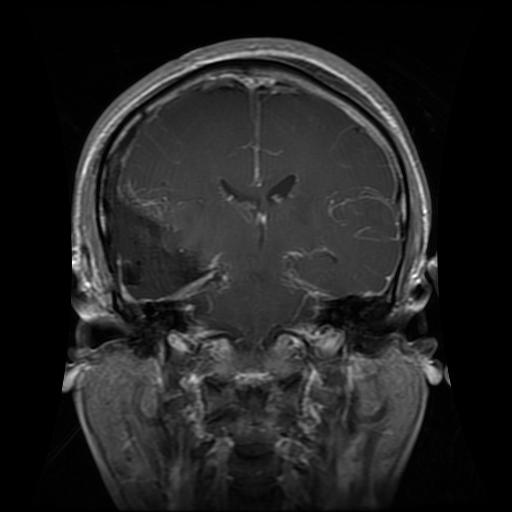
\includegraphics[width=\linewidth,height=3.0cm,keepaspectratio]{legacy/results/mri_examples/glioma.jpg}\\Glioma\end{minipage}\hfill
\begin{minipage}{0.24\textwidth}\centering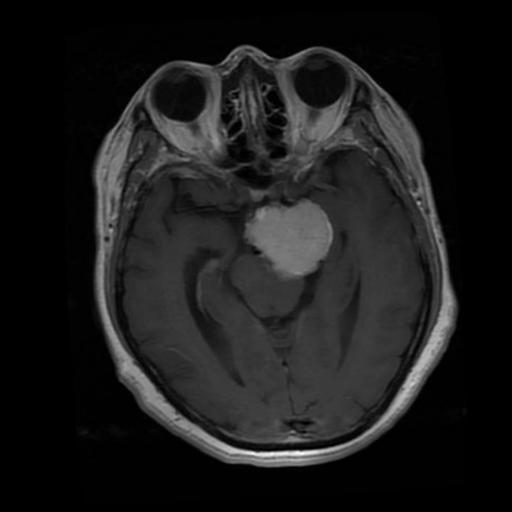
\includegraphics[width=\linewidth,height=3.0cm,keepaspectratio]{legacy/results/mri_examples/meningioma.jpg}\\Meningioma\end{minipage}\hfill
\begin{minipage}{0.24\textwidth}\centering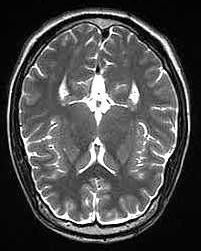
\includegraphics[width=\linewidth,height=3.0cm,keepaspectratio]{legacy/results/mri_examples/notumor.jpg}\\Không u\end{minipage}\hfill
\begin{minipage}{0.24\textwidth}\centering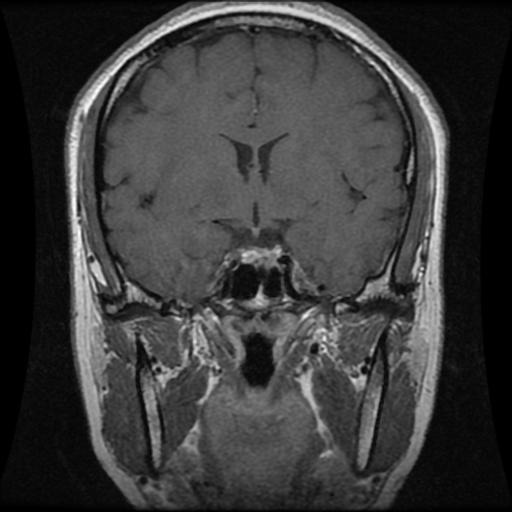
\includegraphics[width=\linewidth,height=3.0cm,keepaspectratio]{legacy/results/mri_examples/pituitary.jpg}\\Pituitary\end{minipage}
\caption{Ví dụ ảnh MRI thuộc bốn nhóm trong bộ dữ liệu của đề tài \citep{dataset}.}\label{fig:mri}
\end{figure}

Những năm gần đây, các mô hình học sâu (\textit{deep learning}) đã đạt kết quả tốt trong phân loại ảnh, và ảnh y tế là một lĩnh vực ứng dụng tiềm năng. Tuy nhiên, các mô hình này cần lượng dữ liệu lớn và đa dạng, trong khi dữ liệu y tế lại nằm rải rác tại từng bệnh viện, phòng khám. Mỗi nơi chỉ có một phần nhỏ dữ liệu, và việc gom chúng về một kho chung gặp nhiều trở ngại về quản trị, đạo đức nghề nghiệp lẫn pháp lý: thông tin về tình trạng sức khỏe thuộc nhóm dữ liệu cá nhân nhạy cảm theo quy định hiện hành của Việt Nam \citep{nd13}.

\begin{figure}[H]\centering
\begin{tikzpicture}[font=\small,>=Latex,box/.style={draw,rounded corners,align=center,minimum width=2.7cm,minimum height=0.9cm},node distance=0.7cm]
\node[box,fill=blue!8] (h1) {Bệnh viện A\\Ảnh MRI};
\node[box,fill=blue!8,right=of h1] (h2) {Bệnh viện B\\Ảnh MRI};
\node[box,fill=orange!15,below=of h1,xshift=1.65cm] (s) {Máy chủ\\mô hình};
\draw[->,thick] (h1)--(s);\draw[->,thick] (h2)--(s);
\node[below=0.15cm of s,font=\footnotesize,align=center] {Tập trung: ảnh được chuyển về máy chủ};
\begin{scope}[xshift=8.3cm]
\node[box,fill=green!10] (c1) {Bệnh viện A\\Ảnh MRI + huấn luyện};
\node[box,fill=green!10,right=of c1] (c2) {Bệnh viện B\\Ảnh MRI + huấn luyện};
\node[box,fill=orange!15,below=of c1,xshift=1.65cm] (g) {Máy chủ\\tổng hợp tham số};
\draw[<->,thick] (c1)--node[left,font=\scriptsize,fill=white]{tham số}(g);
\draw[<->,thick] (c2)--node[right,font=\scriptsize,fill=white]{tham số}(g);
\node[below=0.15cm of g,font=\footnotesize,align=center] {Học liên kết: ảnh ở lại từng nơi};
\end{scope}
\end{tikzpicture}
\caption{Học tập trung và học liên kết: hai cách tổ chức huấn luyện khi dữ liệu nằm ở nhiều nơi.}\label{fig:central}
\end{figure}

Học liên kết (\textit{Federated Learning}, FL) là hướng tiếp cận nhằm giải quyết mâu thuẫn trên. Thay vì gửi ảnh về một nơi, mỗi bên tham gia (\textit{client}) huấn luyện mô hình ngay trên dữ liệu của mình rồi chỉ gửi bản cập nhật tham số cho máy chủ (\textit{server}); máy chủ tổng hợp các cập nhật để được mô hình chung \citep{mcmahan,kairouz}. Hướng đi này đã được đề xuất cho y tế số và được thử nghiệm với bài toán u não \citep{rieke,sheller}.

Tuy vậy, học liên kết không tự động giải quyết mọi vấn đề. Thứ nhất, dữ liệu giữa các bên thường không đồng nhất (\textit{non-IID}): một bệnh viện chuyên khoa có thể gặp một loại u nhiều hơn hẳn các loại khác, khiến mô hình cục bộ bị kéo lệch và việc tổng hợp trở nên khó khăn hơn \citep{zhao,hsieh}. Thứ hai, việc không chia sẻ ảnh gốc chưa bảo đảm rằng bản cập nhật không làm lộ thông tin: nhiều nghiên cứu đã chỉ ra khả năng khôi phục dữ liệu từ gradient hoặc suy đoán một mẫu có nằm trong tập huấn luyện hay không \citep{zhu,shokri}. Quyền riêng tư vi phân (\textit{Differential Privacy}, DP) là khuôn khổ toán học cho phép đo mức ảnh hưởng của từng mẫu lên kết quả huấn luyện, nhưng việc áp dụng DP thường làm giảm độ chính xác của mô hình \citep{dwork,abadi}.

Từ bối cảnh đó, nhóm chúng em xây dựng một hệ thống mô phỏng học liên kết cho bài toán phân loại bốn nhóm ảnh MRI não với bốn client có phân bố nhãn lệch. Hệ thống so sánh bốn cấu hình: FedAvg, FedProx, FedProx kết hợp DP-SGD và FedProx kết hợp DP-SGD với AutoClip, đồng thời khảo sát mức riêng tư và thử một phép tấn công suy luận thành viên. Trong kết quả seed 42, FedAvg đạt accuracy 92,50\% và Macro-F1 92,29\%; FedProx đạt lần lượt 92,19\% và 91,96\%. Hai cấu hình bật DP-SGD đạt accuracy 67,44\% (clipping cố định) và 65,88\% (AutoClip). Đây là kết quả sơ bộ một seed; AutoClip và cơ chế sinh nhiễu hiện chưa đủ căn cứ để khẳng định bảo đảm DP.

\section{Các nghiên cứu có liên quan}
\subsection{Học liên kết và FedAvg}
Trong học liên kết, mô hình toàn cục được cải thiện qua nhiều vòng. Ở mỗi vòng, server gửi mô hình hiện tại cho các client; mỗi client huấn luyện cục bộ vài epoch; server thu các cập nhật và lấy trung bình có trọng số theo số mẫu. Thuật toán FedAvg thực hiện đúng quy trình này và là nền tảng của phần lớn các phương pháp sau đó \citep{mcmahan}. Các tổng quan của Kairouz và cộng sự \citep{kairouz} cho thấy bên cạnh hiệu quả truyền thông, bài toán còn nhiều thách thức mở về tính không đồng nhất của dữ liệu và về quyền riêng tư. Trong y tế, Sheller và cộng sự đã huấn luyện liên kết mô hình phân đoạn u não đa cơ sở mà không chia sẻ dữ liệu bệnh nhân \citep{sheller}, còn Rieke và cộng sự phân tích tiềm năng và các rào cản của hướng đi này \citep{rieke}.

\subsection{Dữ liệu non-IID và FedProx}
Khi phân bố nhãn khác nhau giữa các client, mỗi client tối ưu về một nghiệm riêng, và trung bình các nghiệm đó có thể kém hơn mô hình huấn luyện tập trung; hiện tượng này đã được ghi nhận trong các khảo sát thực nghiệm \citep{zhao,hsieh}. FedProx xử lý một phần vấn đề bằng cách thêm hạng tử phạt khoảng cách tới mô hình toàn cục vào mục tiêu cục bộ, nhờ đó các client không đi quá xa nhau trong mỗi vòng \citep{fedprox}. Ngoài ra, khi mỗi client có phân bố nhãn lệch, hàm mất mát có thể được hiệu chỉnh theo tần suất lớp, như trong Balanced Softmax vốn được đề xuất cho dữ liệu mất cân bằng \citep{ren}. Cần lưu ý FedAvg và FedProx giải quyết vấn đề tối ưu, chứ không phải cơ chế bảo mật dữ liệu.

\subsection{Quyền riêng tư vi phân và DP-SGD}
Quyền riêng tư vi phân yêu cầu kết quả của thuật toán gần như không đổi khi thêm hoặc bớt một mẫu dữ liệu \citep{dwork}. DP-SGD hiện thực ý tưởng này trong huấn luyện mạng nơ-ron bằng cách cắt chuẩn gradient của từng mẫu rồi cộng nhiễu Gauss, kèm một bộ kế toán để theo dõi mức riêng tư tích lũy \citep{abadi}. Bộ kế toán dựa trên độ phân kỳ Rényi cho phép tính chặt hơn khi nhiều bước huấn luyện được hợp lại \citep{mironov17,mironov19}. Mức riêng tư càng chặt (epsilon càng nhỏ) thì nhiễu càng lớn và mô hình thường kém chính xác hơn.

\begin{figure}[H]\centering
\begin{tikzpicture}[font=\small,>=Latex,dp/.style={draw,rounded corners,fill=blue!8,align=center,minimum width=2.6cm,minimum height=1.0cm}]
\node[dp] (a) {Gradient\\từng mẫu};
\node[dp,right=0.55cm of a] (b) {Cắt chuẩn\\$\|g_i\|_2\leq C$};
\node[dp,right=0.55cm of b,fill=orange!15] (c) {Cộng nhiễu\\Gauss};
\node[dp,right=0.55cm of c,fill=green!10] (d) {Cập nhật\\tham số};
\draw[->,thick] (a)--(b);\draw[->,thick] (b)--(c);\draw[->,thick] (c)--(d);
\end{tikzpicture}
\caption{Minh họa các bước chính của DP-SGD.}\label{fig:dpsgd}
\end{figure}

\subsection{Suy luận thành viên}
Tấn công suy luận thành viên (\textit{membership inference}) nhằm đoán một mẫu có thuộc tập huấn luyện hay không, thường dựa trên việc mô hình có xu hướng cho mất mát thấp hơn trên dữ liệu đã thấy \citep{shokri,yeom}. Đây là một phép thử thực nghiệm cho rò rỉ thông tin; kết quả thấp không chứng minh mô hình an toàn. Carlini và cộng sự đề nghị đánh giá thêm tỉ lệ dương thật tại tỉ lệ dương giả rất thấp thay vì chỉ dùng độ chính xác trung bình \citep{carlini}.

\section{Mục tiêu, phạm vi và định vị đề tài}
Mục tiêu của đề tài là triển khai và đánh giá một quy trình học liên kết phân loại bốn nhóm ảnh MRI dưới phân phối non-IID, đồng thời khảo sát đánh đổi giữa hiệu năng và các biện pháp riêng tư. Nghiên cứu trả lời ba câu hỏi: (1) mô hình liên kết đạt hiệu năng ra sao trong thiết lập client lệch nhãn; (2) FedProx có cải thiện so với FedAvg trong các lần chạy đã thực hiện hay không; (3) DP-SGD làm thay đổi hiệu năng và kết quả phép thử suy luận thành viên như thế nào.

Dữ liệu là Brain Tumor MRI Dataset công khai của Nickparvar với bốn lớp, gồm 5.600 ảnh huấn luyện và 1.600 ảnh kiểm tra \citep{dataset}. Bốn client được mô phỏng trên cùng một máy, nên đây không phải kết nối hay đánh giá tại bệnh viện thật. Đề tài không đề xuất thuật toán FL hay DP mới; đóng góp nằm ở việc tích hợp các thành phần đã có, thiết kế phân hoạch lệch nhãn có định lượng, đánh giá có hệ thống và nêu rõ giới hạn của phép thử. Kết quả không suy rộng sang bệnh viện độc lập, máy MRI khác hay quyết định lâm sàng.

% ======================= CHƯƠNG 2 =======================
\chapter{Tóm tắt nghiên cứu}
\section{Kiến trúc hệ thống}
Hệ thống gồm một server và bốn client chạy tuần tự trên cùng một máy; mỗi vòng huấn luyện diễn ra theo bốn bước (Hình~\ref{fig:flow}). Bước (1): server cung cấp mô hình toàn cục $w_r$ của vòng $r$. Bước (2): mỗi client nạp $w_r$ và huấn luyện trên ảnh cục bộ. Bước (3): client gửi lại \emph{độ lệch tham số} $\Delta_k$ so với $w_r$, không gửi ảnh. Bước (4): server kiểm tra tính hợp lệ của các cập nhật và tổng hợp thành $w_{r+1}$. Việc trao đổi được mô phỏng qua một thư mục dùng chung, nên minh họa đúng giao diện giữa các bên nhưng không tạo ra sự cô lập hạ tầng thật.

\begin{figure}[H]\centering
\begin{tikzpicture}[font=\small,>=Latex,
 box/.style={draw,rounded corners,align=center,minimum height=1.2cm,text width=3cm,fill=gray!8},
 client/.style={draw,rounded corners,align=center,minimum height=0.9cm,text width=2.5cm,fill=blue!6},
 arr/.style={->,thick}]
\node[box] (g) at (0,0) {Mô hình toàn cục\\$w_r$};
\node[client] (a) at (5.4,2.7)  {Client A\\[-1pt]{\footnotesize ảnh cục bộ}};
\node[client] (b) at (5.4,0.9)  {Client B\\[-1pt]{\footnotesize ảnh cục bộ}};
\node[client] (c) at (5.4,-0.9) {Client C\\[-1pt]{\footnotesize ảnh cục bộ}};
\node[client] (d) at (5.4,-2.7) {Client D\\[-1pt]{\footnotesize ảnh cục bộ}};
\node[box,text width=4.3cm] (s) at (11.6,0) {Server: kiểm tra\\và tổng hợp\\[2pt]$w_{r+1}=w_r+\sum_k p_k\Delta_k$};
\foreach \x in {a,b,c,d}{\draw[arr](g.east)--(\x.west);\draw[arr](\x.east)--(s.west);}
\node[font=\footnotesize] at (2.2,2.3) {(1) gửi $w_r$};
\node[font=\footnotesize] at (8.6,2.3) {(3) gửi $\Delta_k$};
\draw[arr](s.south)--(11.6,-4.0)--(0,-4.0)--(g.south);
\node[font=\footnotesize,fill=white,inner sep=2pt] at (5.6,-4.0) {(4) mô hình của vòng kế tiếp};
\node[font=\footnotesize] at (5.4,3.6) {(2) huấn luyện cục bộ};
\end{tikzpicture}
\caption{Luồng huấn luyện liên kết mô phỏng. Gói cập nhật chứa độ lệch tham số, không chứa ảnh gốc.}\label{fig:flow}
\end{figure}

\section{Cơ sở toán học của phương pháp}
\subsection{Bài toán tối ưu liên kết}
Gọi $K=4$ là số client, $\Dk$ là tập dữ liệu của client $k$ với $n_k=|\Dk|$ và $n=\sum_k n_k$. Với mô hình $f(\cdot;w)$ và hàm mất mát $\ell$, mất mát cục bộ và mục tiêu toàn cục là
\[
F_k(w)=\frac{1}{n_k}\sum_{(x,y)\in\Dk}\ell\bigl(f(x;w),y\bigr),\qquad
F(w)=\sum_{k=1}^{K}p_kF_k(w),\quad p_k=\frac{n_k}{n}.
\]
Do $\nabla F=\sum_k p_k\nabla F_k$ tại cùng một điểm $w$, nếu mỗi client chỉ làm một bước gradient thì trung bình có trọng số các cập nhật bằng đúng một bước gradient trên toàn bộ dữ liệu. Khi mỗi client làm nhiều bước cục bộ trên phân bố riêng $P_k(x,y)\neq P(x,y)$, quỹ đạo của chúng tách khỏi nhau, một hiện tượng gọi là \emph{trôi client} (\textit{client drift}). Đó là lý do dữ liệu non-IID làm giảm chất lượng của FedAvg.

\subsection{FedAvg và FedProx}
FedProx thay mục tiêu cục bộ bằng
\[
h_k(w;w_r)=F_k(w)+\frac{\mu}{2}\norm{w-w_r}_2^2,\qquad
\nabla h_k(w;w_r)=\nabla F_k(w)+\mu\,(w-w_r).
\]
Một bước gradient với tốc độ học $\eta$ cho $w\leftarrow(1-\eta\mu)\,w+\eta\mu\,w_r-\eta\nabla F_k(w)$: ngoài gradient của dữ liệu, tham số còn bị kéo về $w_r$ với cường độ $\eta\mu$, nên quãng đường client có thể trôi bị hạn chế. Với $\mu=0$ ta được FedAvg. Chỉ một tập con tham số $\theta$ được huấn luyện (phần còn lại bị đóng băng); client $k$ gửi $\Delta_k=\theta_k-\theta_r$ và server cập nhật
\[
\theta_{r+1}=\theta_r+\sum_{k}p_k\Delta_k=\sum_k p_k\theta_k,
\]
vì $\sum_kp_k=1$; tức là tổng hợp độ lệch tương đương với lấy trung bình có trọng số các tham số cục bộ. Do bốn client có cùng 1.200 ảnh, ta có $p_k=1/4$.

\subsection{Hiệu chỉnh mất mát theo tần suất lớp}
Khi client $k$ có tần suất lớp $\pi_k(c)$ lệch, với giả thiết dịch chuyển nhãn ($p(x\mid c)$ giống nhau giữa các client), quy tắc Bayes cho
\[
p_k(y=c\mid x)=\frac{\pi_k(c)\,p(x\mid c)}{\sum_{j}\pi_k(j)\,p(x\mid j)}.
\]
Mạng sẽ học hậu nghiệm bị thiên lệch bởi $\pi_k$. Balanced Softmax bù lại bằng cách cộng $\log\hat\pi_k(c)$ vào logit $z_c$ trước khi tính mất mát:
\[
\ell_{\mathrm{BS}}=-\log\frac{\hat\pi_k(y)\,e^{z_y}}{\sum_{c}\hat\pi_k(c)\,e^{z_c}},\qquad
\hat\pi_k(c)=\frac{n_{k,c}+1}{n_k+C},
\]
trong đó $C=4$ là số lớp và tử số $+1$ là làm mượt Laplace để tránh $\log 0$. Khi đó $z_c$ chủ yếu mô hình hóa phần $p(x\mid c)$ dùng chung giữa các client, thay vì phần tần suất riêng của từng nơi.

\subsection{DP-SGD và kế toán riêng tư}\label{sec:dp}
Một thuật toán ngẫu nhiên $\mathcal M$ là $(\varepsilon,\delta)$-DP nếu với mọi cặp tập dữ liệu kề nhau $D,D'$ (khác nhau một mẫu) và mọi tập kết quả $S$: $\Pr[\mathcal M(D)\in S]\le e^{\varepsilon}\Pr[\mathcal M(D')\in S]+\delta$ \citep{dwork}. Với gradient từng mẫu $g_i$ và ngưỡng $C$, DP-SGD tính
\[
\bar g_i=g_i\cdot\min\!\Bigl(1,\frac{C}{\norm{g_i}_2}\Bigr),\qquad
\widetilde g=\frac{1}{B}\Bigl[\sum_{i=1}^{B}\bar g_i+\mathcal N\bigl(0,\sigma^2C^2I\bigr)\Bigr],
\]
với $B$ là kích thước batch kỳ vọng và $\sigma$ là hệ số nhiễu. Sau khi cắt, $\norm{\bar g_i}_2\le C$, nên tổng có độ nhạy $\ell_2$ bằng $C$ khi thêm hoặc bớt một mẫu. Cơ chế Gauss với độ lệch chuẩn $\sigma C$ thỏa $(\alpha,\alpha/2\sigma^2)$-RDP cho mỗi bước khi không lấy mẫu con; lấy mẫu Poisson tỉ lệ $q=B/n_k$ làm giảm đáng kể giá trị này \citep{mironov19}. RDP cộng dồn qua $T$ bước và được đổi sang $(\varepsilon,\delta)$-DP theo công thức \citep{mironov17}:
\[
\varepsilon=\min_{\alpha>1}\Bigl[T\,\varepsilon_{\mathrm{bước}}(\alpha)+\frac{\log(1/\delta)}{\alpha-1}\Bigr]
\]
Vì $\Delta_k$ chỉ là hàm của các gradient đã làm nhiễu, tính chất hậu xử lý bảo đảm bước tổng hợp tại server không làm yếu mức riêng tư vừa tính. Cần lưu ý đây là bảo vệ ở mức mẫu, và bộ kế toán trong đề tài là phần tự cài đặt (xem mục~\ref{sec:hanche}).

Một đánh giá định lượng giúp dự đoán chi phí hiệu năng: nhiễu có $\E\norm{\mathcal N(0,\sigma^2C^2I)/B}_2^2=\sigma^2C^2d/B^2$, trong khi tín hiệu có chuẩn tối đa $C$. Với $d=1.239.588$ tham số huấn luyện, $\sigma=C=1$ và $B=32$, chuẩn nhiễu kỳ vọng xấp xỉ $\sqrt d/B\approx 34{,}8$, lớn hơn nhiều lần so với cận trên $C=1$ của tín hiệu. Mỗi bước vì thế có tỉ số tín hiệu trên nhiễu thấp, và chỉ nhiễu trung bình dần qua nhiều bước mới giúp mô hình hội tụ.

\section{Dữ liệu và phân hoạch non-IID}
Từ 5.600 ảnh huấn luyện, chúng em giữ lại 100 ảnh mỗi lớp (400 ảnh) làm tập kiểm định toàn cục, chọn 4.800 ảnh cho bốn client (1.200 ảnh mỗi client) và 400 ảnh còn lại không thuộc client nào. Tập kiểm tra gồm 1.600 ảnh, mỗi lớp 400 ảnh. Mỗi client nhận 840 ảnh (70\%) thuộc một lớp chủ đạo và 120 ảnh (10\%) cho mỗi lớp còn lại; lớp chủ đạo của bốn client lần lượt là glioma, meningioma, notumor và pituitary (Hình~\ref{fig:noniid}). Hợp của bốn client có phân bố đều (25\% mỗi lớp), nhưng từng client lệch rõ rệt: khoảng cách biến thiên toàn phần so với phân bố đều là $\mathrm{TV}=\tfrac12\sum_c|\pi_k(c)-\tfrac14|=0{,}45$ và độ phân kỳ $\mathrm{KL}(\pi_k\Vert U)=0{,}7\ln\tfrac{0{,}7}{0{,}25}+0{,}3\ln\tfrac{0{,}1}{0{,}25}\approx0{,}446$ nat. Đây là mức lệch nhãn mạnh nhưng vẫn giữ đủ ảnh của mọi lớp ở mỗi client.

\newcommand{\rowbar}[6]{% #1 y, #2 nhãn, #3..#6 tỉ lệ bốn lớp
 \pgfmathsetmacro{\xa}{#3*7}\pgfmathsetmacro{\xb}{(#3+#4)*7}\pgfmathsetmacro{\xc}{(#3+#4+#5)*7}
 \fill[red!45]    (0,#1) rectangle (\xa,#1+0.55);
 \fill[blue!35]   (\xa,#1) rectangle (\xb,#1+0.55);
 \fill[green!40]  (\xb,#1) rectangle (\xc,#1+0.55);
 \fill[orange!50] (\xc,#1) rectangle (7,#1+0.55);
 \draw (0,#1) rectangle (7,#1+0.55);
 \node[left,font=\footnotesize] at (0,#1+0.275) {#2};
 \pgfmathsetmacro{\ma}{\xa/2}\pgfmathsetmacro{\mb}{(\xa+\xb)/2}\pgfmathsetmacro{\mc}{(\xb+\xc)/2}\pgfmathsetmacro{\md}{(\xc+7)/2}
 \pgfmathtruncatemacro{\pa}{round(#3*100)}\node[font=\scriptsize] at (\ma,#1+0.275) {\pa\%};
 \pgfmathtruncatemacro{\pb}{round(#4*100)}\node[font=\scriptsize] at (\mb,#1+0.275) {\pb\%};
 \pgfmathtruncatemacro{\pc}{round(#5*100)}\node[font=\scriptsize] at (\mc,#1+0.275) {\pc\%};
 \pgfmathtruncatemacro{\pd}{round(#6*100)}\node[font=\scriptsize] at (\md,#1+0.275) {\pd\%};}
\begin{figure}[H]\centering
\begin{tikzpicture}[x=1cm,y=1cm]
\rowbar{2.4}{Client A}{0.7}{0.1}{0.1}{0.1}
\rowbar{1.6}{Client B}{0.1}{0.7}{0.1}{0.1}
\rowbar{0.8}{Client C}{0.1}{0.1}{0.7}{0.1}
\rowbar{0.0}{Client D}{0.1}{0.1}{0.1}{0.7}
\fill[red!45] (0.5,-0.9) rectangle (0.8,-0.65);\node[right,font=\scriptsize] at (0.8,-0.775){Glioma};
\fill[blue!35] (2.2,-0.9) rectangle (2.5,-0.65);\node[right,font=\scriptsize] at (2.5,-0.775){Meningioma};
\fill[green!40] (4.4,-0.9) rectangle (4.7,-0.65);\node[right,font=\scriptsize] at (4.7,-0.775){Không u};
\fill[orange!50] (5.9,-0.9) rectangle (6.2,-0.65);\node[right,font=\scriptsize] at (6.2,-0.775){Pituitary};
\end{tikzpicture}
\caption{Phân bố nhãn của bốn client: mỗi client có một lớp chủ đạo chiếm 70\% số ảnh.}\label{fig:noniid}
\end{figure}

\section{Xây dựng hệ thống thử nghiệm}
Mô hình nền là MobileNetV3-Small khởi tạo từ trọng số huấn luyện trước trên ImageNet \citep{howard,deng}. Đây là kiến trúc nhẹ nên phù hợp với việc truyền cập nhật qua nhiều vòng. Chúng em chỉ huấn luyện các khối cuối của backbone và bộ phân loại ($d=1.239.588$ tham số); các khối còn lại bị đóng băng và lớp chuẩn hóa batch được giữ ở chế độ đánh giá, nên thống kê chuẩn hóa không bị cập nhật theo dữ liệu cục bộ lệch. Ảnh được đưa về RGB kích thước $224\times224$, có tăng cường dữ liệu nhẹ khi huấn luyện (Hình~\ref{fig:arch}).

\begin{figure}[H]\centering
\begin{tikzpicture}[font=\small,>=Latex,net/.style={draw,rounded corners,align=center,minimum height=1.0cm}]
\node[net,fill=gray!15,minimum width=3.5cm] (a) {Ảnh MRI\\$224\times224$};
\node[net,fill=blue!10,minimum width=4.2cm,right=0.5cm of a] (b) {MobileNetV3-Small\\các khối đầu đóng băng};
\node[net,fill=orange!15,minimum width=4.1cm,right=0.5cm of b] (c) {Các khối cuối\\được huấn luyện};
\node[net,fill=green!10,minimum width=3.2cm,right=0.5cm of c] (d) {Phân loại\\4 lớp};
\draw[->,thick] (a)--(b);\draw[->,thick] (b)--(c);\draw[->,thick] (c)--(d);
\end{tikzpicture}
\caption{Phần mạng bị đóng băng và phần được huấn luyện trong mỗi vòng liên kết.}\label{fig:arch}
\end{figure}

Quy trình thực nghiệm gồm 20 vòng, mỗi client huấn luyện 3 epoch mỗi vòng với batch 32 và tốc độ học $10^{-4}$, dùng Balanced Softmax và $\mu=0{,}01$ cho FedProx (FedAvg ứng với $\mu=0$). Cấu hình DP dùng $\sigma=1$, $C=1$ và $\delta=10^{-5}$. Sau mỗi vòng, mô hình được đánh giá trên tập kiểm định; vòng có Macro-F1 kiểm định cao nhất được chọn và chỉ vòng đó được đo trên tập kiểm tra. Server kiểm tra số vòng, số mẫu, kích thước tensor và giá trị hữu hạn của mỗi cập nhật; đây chỉ là kiểm tra toàn vẹn cơ bản, chưa thay thế xác thực danh tính, mã hóa kênh truyền hay tổng hợp an toàn (\textit{secure aggregation}). Thí nghiệm chạy trên GPU NVIDIA T4 (Google Colab).

% ======================= CHƯƠNG 3 =======================
\chapter{Kết quả sơ bộ}
\section{Thiết kế đánh giá}
Với $N$ ảnh kiểm tra và $C$ lớp, accuracy là tỉ lệ dự đoán đúng; với mỗi lớp $c$, recall $R_c=\mathrm{TP}_c/(\mathrm{TP}_c+\mathrm{FN}_c)$, precision $P_c=\mathrm{TP}_c/(\mathrm{TP}_c+\mathrm{FP}_c)$ và $F1_c=2P_cR_c/(P_c+R_c)$. Macro-F1 là trung bình cộng các $F1_c$, còn balanced accuracy là trung bình cộng các $R_c$. Vì accuracy bằng $\sum_c (N_c/N)R_c$ và tập kiểm tra có $N_c=N/C$ ảnh mỗi lớp, hai chỉ số này trùng nhau trong thí nghiệm. Bảng dưới đây là kết quả sơ bộ của seed 42 với cấu hình fine-tune các block cuối ($d=1.239.588$). Tệp tổng hợp hiện chỉ có một seed, nên độ lệch chuẩn mẫu chưa xác định và không được suy diễn từ bảng này. Notebook hợp nhất bổ sung thí nghiệm riêng với classifier cuối (`linear`, khoảng 4 nghìn tham số), ba seed và thanh sai số; các kết quả đó chỉ được đưa vào báo cáo sau khi chạy đủ và kiểm tra dữ liệu đầu ra.

\section{Hiệu năng của bốn cấu hình}
\begin{table}[H]\centering
\scriptsize
\begin{tabularx}{\textwidth}{Xrrrrrr}
\toprule
\textbf{Cấu hình} & \textbf{Vòng} & \textbf{Val acc.} & \textbf{Val F1} & \textbf{Test acc.} & \textbf{Test F1} & \textbf{Test bal. acc.}\\
\midrule
FedAvg & 18 & 95,75\% & 95,74\% & 92,50\% & 92,29\% & 92,50\%\\
FedProx ($\mu=0{,}01$) & 18 & 96,00\% & 95,99\% & 92,19\% & 91,96\% & 92,19\%\\
FedProx + DP-SGD & 18 & 74,50\% & 72,89\% & 67,44\% & 64,74\% & 67,44\%\\
FedProx + DP-SGD + AutoClip (thăm dò) & 20 & 72,50\% & 70,27\% & 65,88\% & 63,19\% & 65,88\%\\
\bottomrule
\end{tabularx}
\caption{Kết quả kiểm định và kiểm tra theo seed 42; vòng chọn theo Macro-F1 kiểm định. Các giá trị được làm tròn đến hai chữ số thập phân.}\label{tab:main}
\end{table}

Trong lần chạy sơ bộ seed 42, FedAvg/FedProx đạt accuracy 92,50\%/92,19\%; hai cấu hình DP đạt 67,44\%/65,88\%. Đây là so sánh mô tả trên cấu hình fine-tune các block cuối, chưa phải ước lượng ổn định qua nhiều seed. Notebook mới kiểm tra riêng giả thuyết chỉ huấn luyện classifier cuối; chưa có kết quả chạy mới để kết luận mức accuracy được cải thiện.

\begin{figure}[H]\centering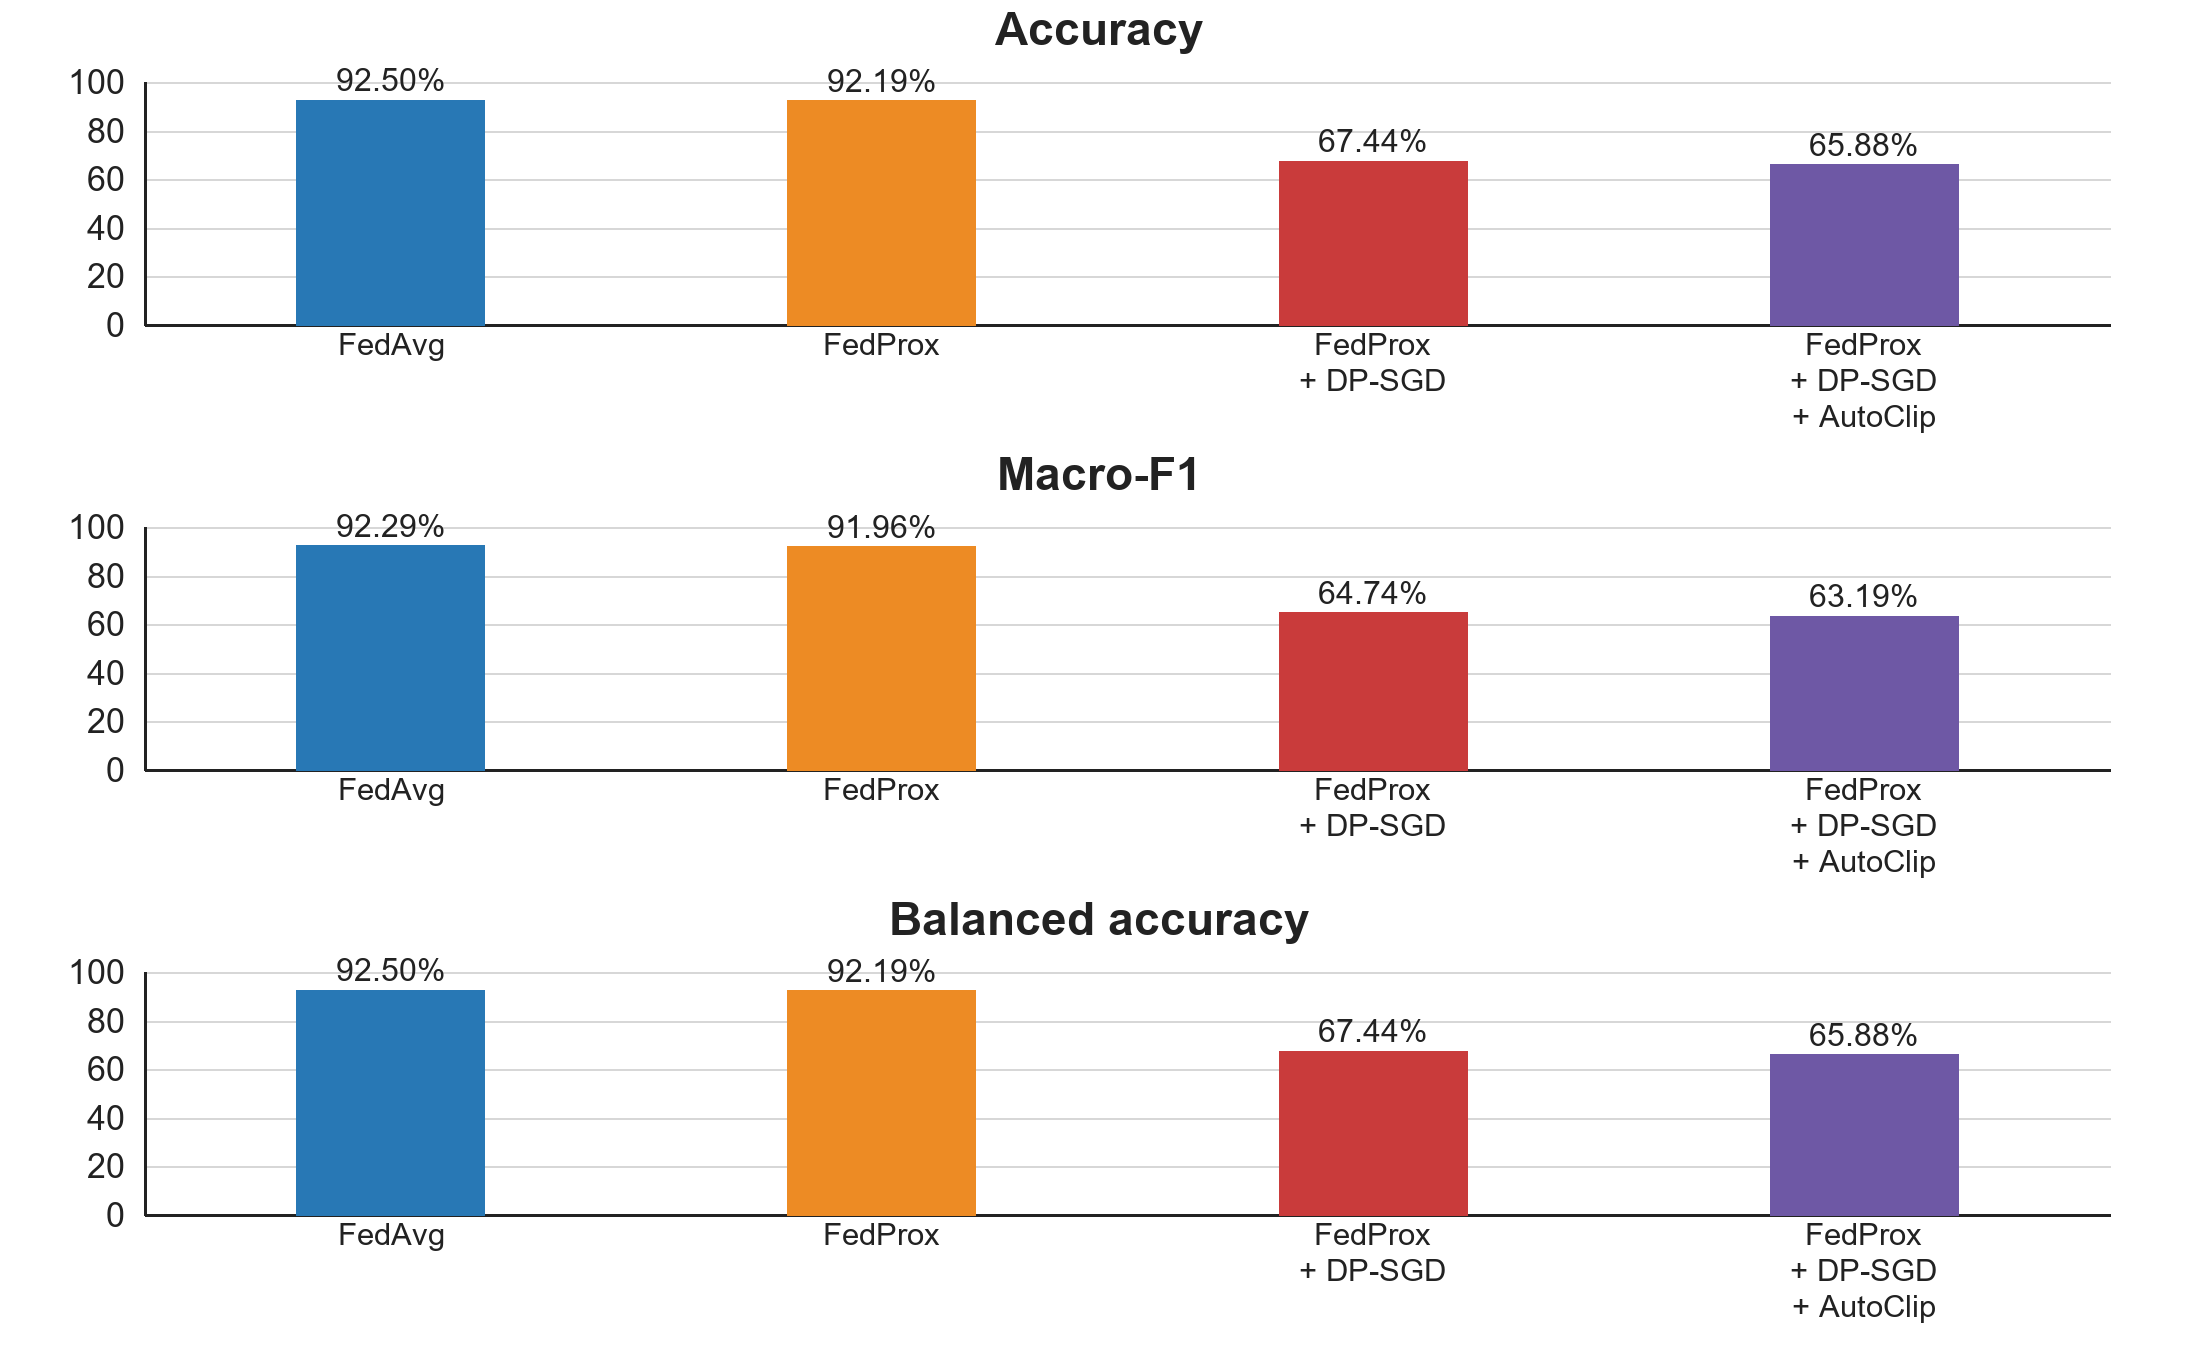
\includegraphics[width=.98\textwidth,height=9cm,keepaspectratio]{legacy/results/report_priority1.png}
\caption{Kết quả sơ bộ seed 42 trên cấu hình fine-tune các block cuối; hình hiện tại chưa có thanh sai số. Notebook tổng hợp mới tạo hình mean $\pm$ std khi đủ ba seed cho từng cấu hình classifier-only.}\label{fig:main}
\end{figure}

\begin{figure}[H]\centering
\begin{minipage}{0.24\textwidth}\centering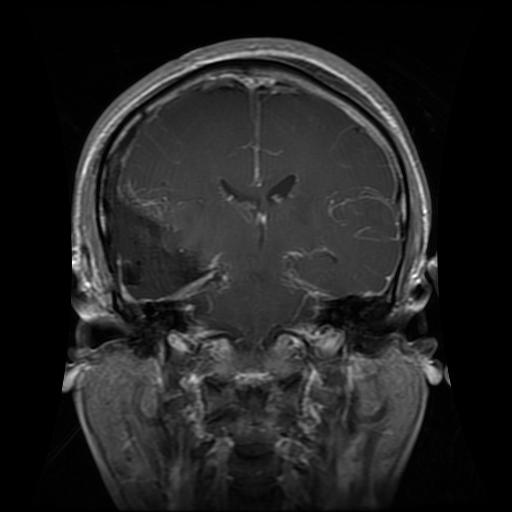
\includegraphics[width=\linewidth,height=2.6cm,keepaspectratio]{legacy/results/mri_examples/glioma.jpg}\\Glioma\end{minipage}\hfill
\begin{minipage}{0.24\textwidth}\centering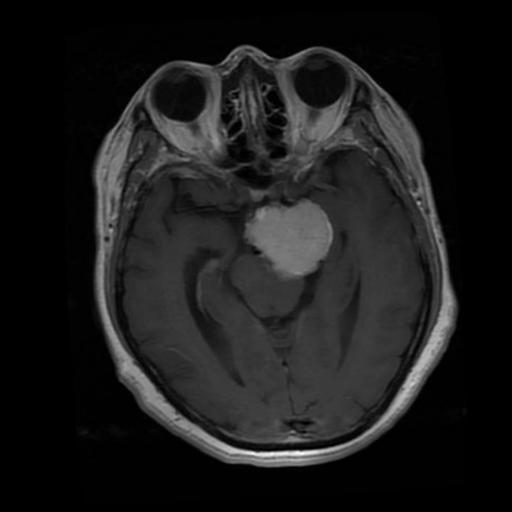
\includegraphics[width=\linewidth,height=2.6cm,keepaspectratio]{legacy/results/mri_examples/meningioma.jpg}\\Meningioma\end{minipage}\hfill
\begin{minipage}{0.24\textwidth}\centering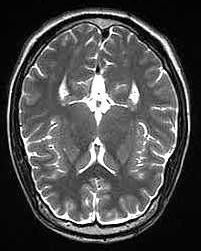
\includegraphics[width=\linewidth,height=2.6cm,keepaspectratio]{legacy/results/mri_examples/notumor.jpg}\\Không u\end{minipage}\hfill
\begin{minipage}{0.24\textwidth}\centering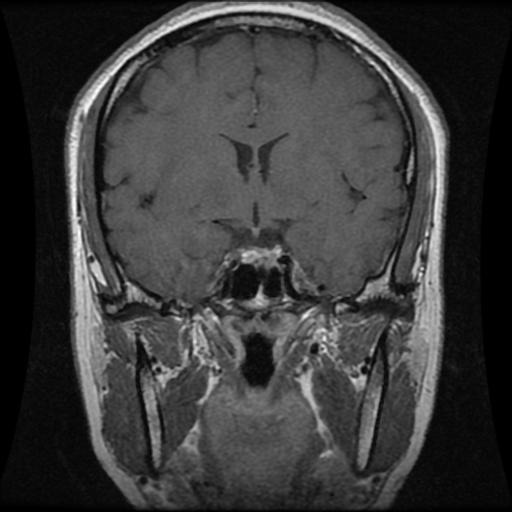
\includegraphics[width=\linewidth,height=2.6cm,keepaspectratio]{legacy/results/mri_examples/pituitary.jpg}\\Pituitary\end{minipage}
\caption*{Ảnh mẫu thuộc bốn lớp của bộ dữ liệu Kaggle; đây là ảnh minh họa dữ liệu, không phải dự đoán của mô hình \citep{dataset}.}
\end{figure}

\begin{figure}[H]\centering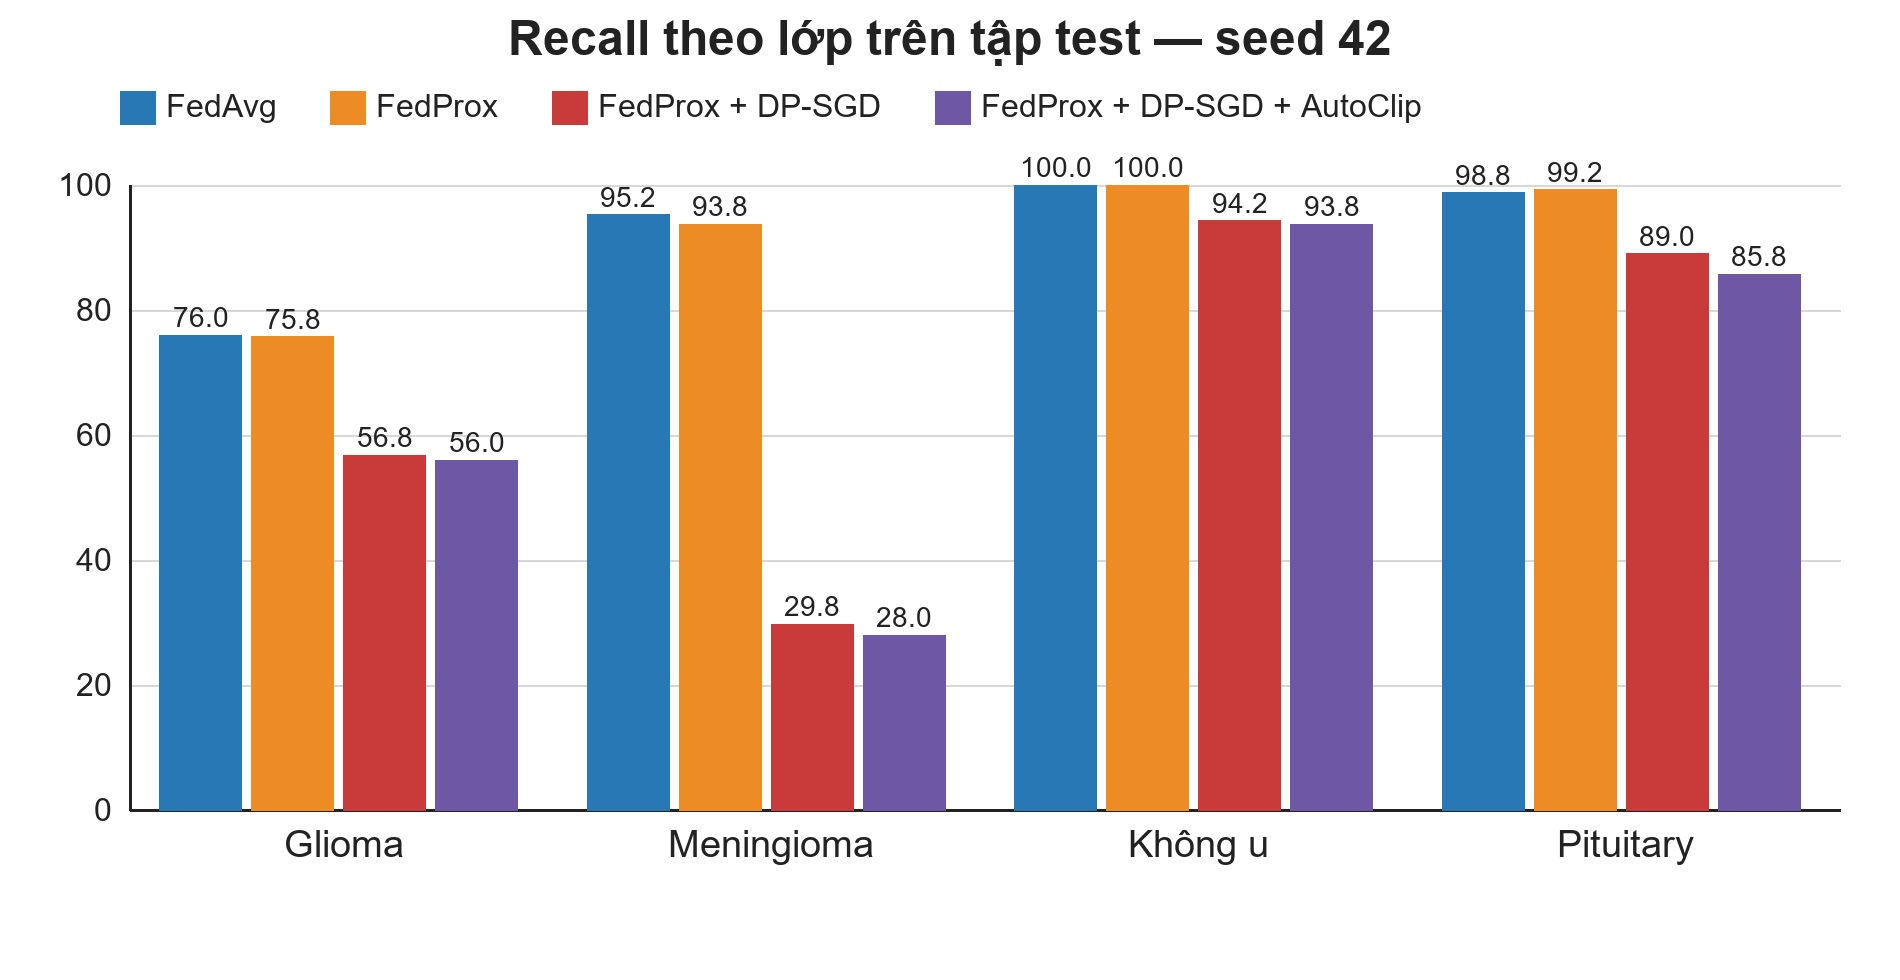
\includegraphics[width=.98\textwidth,height=8cm,keepaspectratio]{legacy/results/report_recall.png}
\caption{Recall theo lớp trên tập kiểm tra cho bốn cấu hình (seed 42).}\label{fig:recall}
\end{figure}

\begin{table}[H]\centering
\begin{tabular}{lrrrr}\toprule
\textbf{Cấu hình} & \textbf{Glioma} & \textbf{Meningioma} & \textbf{Không u} & \textbf{Pituitary}\\\midrule
FedAvg & 76,00\% & 95,25\% & 100,00\% & 98,75\%\\
FedProx & 75,75\% & 93,75\% & 100,00\% & 99,25\%\\
FedProx + DP-SGD & 56,75\% & 29,75\% & 94,25\% & 89,00\%\\
FedProx + DP-SGD + AutoClip & 56,00\% & 28,00\% & 93,75\% & 85,75\%\\\bottomrule
\end{tabular}
\caption{Recall từng lớp trên tập kiểm tra.}\label{tab:recall}
\end{table}

Suy giảm ở hai cấu hình DP tập trung rõ ở meningioma: recall lần lượt là 29,75\% và 28,00\%, trong khi notumor vẫn đạt 94,25\% và 93,75\%. Vì vậy chỉ nhìn accuracy tổng thể có thể bỏ sót lỗi tập trung ở một lớp, điều đặc biệt đáng quan tâm với bài toán y tế.

\section{Khảo sát mức riêng tư}
Một khảo sát sơ bộ trước đây dùng ba epsilon mục tiêu 1, 2 và 3 ($\delta=10^{-5}$, seed 42), nhưng cách áp dụng mục tiêu theo từng vòng không khớp với ngân sách tích lũy toàn run; vì vậy không dùng các số liệu đó để kết luận.

\noindent Bảng và hình sweep epsilon trước đây đã được chuyển khỏi phần kết quả. Chúng dùng \texttt{target\_epsilon} cho từng vòng huấn luyện, trong khi epsilon được cộng dồn qua tất cả các vòng, nên cột mục tiêu không đại diện ngân sách toàn run. Mã đã được sửa để giải σ theo ngân sách tích lũy toàn run và clipping cố định; cần chạy lại ba mức mục tiêu trước khi báo cáo đường cong privacy--utility. AutoClip không nằm trong sweep này vì bước hiệu chỉnh clipping hiện chưa được tính vào privacy accountant.

\section{Thử nghiệm suy luận thành viên}
Kẻ tấn công dùng ngưỡng mất mát $\tau$: dự đoán ``thành viên'' nếu $\ell(x,y)<\tau$. AUC của phép thử là $\Pr[\ell_{\text{ngoài}}>\ell_{\text{trong}}]$ (cộng một nửa xác suất hòa), bằng 0,5 khi tấn công không hơn đoán ngẫu nhiên. Chúng em đo thêm độ chênh mất mát trung bình giữa hai nhóm, độ chính xác tấn công tốt nhất và tỉ lệ dương thật tại tỉ lệ dương giả 1\% (TPR@1\%FPR) \citep{carlini}. Kết quả MIA lưu sẵn trước đây dùng 5.200 ảnh làm thành viên, gồm cả 400 ảnh không được phân vào client; vì vậy bảng và hình MIA hiện tại không hợp lệ để diễn giải. Mã \texttt{mia\_eval.py} đã được sửa để lấy đúng hợp các manifest client (4.800 ảnh theo phân hoạch hiện tại), loại trùng và kiểm tra không giao với tập Testing. Cần chạy lại notebook để tạo bảng/hình MIA đã hiệu chỉnh trước khi dùng kết quả.

\noindent Các số AUC, loss gap và hình MIA trước đây đã được chuyển khỏi phần kết quả vì tập thành viên chứa nhầm 400 ảnh chưa được phân cho client. Sau khi chạy lại notebook với manifest đã sửa, cần bổ sung bảng và hình từ \texttt{runs/p3\_mia.csv} và \texttt{runs/p3\_mia.png}. Hiện chưa có kết quả MIA đã hiệu chỉnh trong báo cáo.

\section{Thảo luận và hạn chế}\label{sec:hanche}
Trong lần chạy sơ bộ seed 42 với 1.239.588 tham số huấn luyện, FedAvg/FedProx đạt accuracy 92,50\%/92,19\% và cấu hình clipping cố định/AutoClip đạt 67,44\%/65,88\%. Đây chỉ ra trade-off trong thiết lập đó; giả thuyết rằng số tham số lớn làm nhiễu lấn át tín hiệu chưa được chứng minh nhân quả. Thiết kế classifier-only trong notebook mới giúp kiểm tra giả thuyết này một cách có kiểm soát, nhưng cần hoàn tất chạy đa seed trước khi kết luận. Các hạn chế hiện tại gồm:
\begin{itemize}
\item Kết quả có sẵn mới gồm seed 42; chưa có 3 seed hoàn chỉnh, vì vậy chưa thể báo cáo mean $\pm$ std hoặc thanh sai số có ý nghĩa.
\item Mỗi client là một phân hoạch nhân tạo của cùng tập dữ liệu công khai, không đại diện cho cơ sở y tế độc lập; chưa có kiểm tra trùng lặp ảnh giữa các phần.
\item Bộ kế toán DP là phần tự cài đặt; lấy mẫu Poisson dùng entropy hệ điều hành nhưng nhiễu Gauss do PyTorch PRNG sinh, chưa phải luồng ngẫu nhiên mật mã đã kiểm định; các giả định này cần được kiểm toán độc lập trước khi nêu bảo đảm riêng tư. Tần suất lớp dùng cho Balanced Softmax chưa được DP bảo vệ, và bước hiệu chỉnh clipping thích nghi cũng chưa được tính vào phân tích riêng tư.
\item Bảng MIA có sẵn gán nhầm 400 ảnh chưa thuộc client là thành viên; mã đã được sửa nhưng phải chạy lại để thay số liệu cũ. Phép thử hiện cũng chỉ dùng loss, một checkpoint và một seed. Mô hình chỉ phân loại ảnh, không định vị tổn thương và chưa được bác sĩ đánh giá.
\end{itemize}

\section{Kết luận và hướng phát triển}
Đề tài đã xây dựng hệ thống mô phỏng học liên kết bốn client với phân bố nhãn lệch có định lượng, so sánh bốn cấu hình và khảo sát thêm mức riêng tư cùng phép thử suy luận thành viên. Ở seed 42, FedAvg đạt 92,50\% accuracy và 92,29\% Macro-F1; FedProx đạt 92,19\% và 91,96\%; FedProx + DP-SGD đạt 67,44\% và 64,74\%; cấu hình AutoClip đạt 65,88\% và 63,19\%. Các kết quả đa seed, classifier-only và MIA đã hiệu chỉnh chưa được chạy trong môi trường hiện tại do bộ dữ liệu không có trong thư mục dự án. Do đó chưa có ước lượng biến thiên giữa seed hoặc bằng chứng rằng DP đạt accuracy mục tiêu. Mục tiêu triển khai và khảo sát mới hoàn thành ở mức mô phỏng sơ bộ; xác nhận bảo đảm riêng tư cần đối chiếu accountant, sampling và bộ sinh ngẫu nhiên. Thuật toán nền, mô hình huấn luyện trước, bộ dữ liệu và thư viện là các thành phần kế thừa.

Hướng tiếp theo là xác minh kết quả của ba seed và tính lại trung bình $\pm$ độ lệch chuẩn; đối chiếu bộ kế toán với một thư viện DP đã được kiểm chứng, dùng nguồn ngẫu nhiên và cơ chế lấy mẫu phù hợp giả định; đánh giá nhiều mức non-IID, bảo vệ siêu dữ liệu nhạy cảm, tổng hợp an toàn và dữ liệu đa cơ sở phân tách theo bệnh nhân. Mọi tuyên bố hướng tới ứng dụng cần được đánh giá chuyên môn y tế trước.

% ======================= CHƯƠNG 4 =======================
\chapter{Tham khảo}
\begin{thebibliography}{99}
\bibitem{dataset} M. Nickparvar. \newblock Brain Tumor MRI Dataset. Kaggle. \newblock DOI: 10.34740/KAGGLE/DSV/2645886. \newblock \url{https://www.kaggle.com/datasets/masoudnickparvar/brain-tumor-mri-dataset}.
\bibitem{nd13} Chính phủ nước Cộng hòa xã hội chủ nghĩa Việt Nam. \newblock Nghị định số 13/2023/NĐ-CP ngày 17/4/2023 về bảo vệ dữ liệu cá nhân.
\bibitem{mcmahan} B. McMahan, E. Moore, D. Ramage, S. Hampson và B. A. y Arcas. \newblock Communication-Efficient Learning of Deep Networks from Decentralized Data. \newblock Proceedings of the 20th International Conference on Artificial Intelligence and Statistics, PMLR 54, tr. 1273--1282, 2017.
\bibitem{kairouz} P. Kairouz và cộng sự. \newblock Advances and Open Problems in Federated Learning. \newblock Foundations and Trends in Machine Learning, 14(1--2):1--210, 2021.
\bibitem{rieke} N. Rieke và cộng sự. \newblock The future of digital health with federated learning. \newblock npj Digital Medicine, 3:119, 2020.
\bibitem{sheller} M. J. Sheller và cộng sự. \newblock Federated learning in medicine: facilitating multi-institutional collaborations without sharing patient data. \newblock Scientific Reports, 9:12598, 2019.
\bibitem{zhao} Y. Zhao, M. Li, L. Lai, N. Suda, D. Civin và V. Chandra. \newblock Federated Learning with Non-IID Data. \newblock arXiv:1806.00582, 2018.
\bibitem{hsieh} K. Hsieh, A. Phanishayee, O. Mutlu và P. Gibbons. \newblock The Non-IID Data Quagmire of Decentralized Machine Learning. \newblock Proceedings of the 37th International Conference on Machine Learning, PMLR 119, tr. 4387--4398, 2020.
\bibitem{zhu} L. Zhu, Z. Liu và S. Han. \newblock Deep Leakage from Gradients. \newblock Advances in Neural Information Processing Systems 32, 2019.
\bibitem{shokri} R. Shokri, M. Stronati, C. Song và V. Shmatikov. \newblock Membership Inference Attacks Against Machine Learning Models. \newblock IEEE Symposium on Security and Privacy, tr. 3--18, 2017.
\bibitem{dwork} C. Dwork và A. Roth. \newblock The Algorithmic Foundations of Differential Privacy. \newblock Foundations and Trends in Theoretical Computer Science, 9(3--4):211--407, 2014.
\bibitem{abadi} M. Abadi và cộng sự. \newblock Deep Learning with Differential Privacy. \newblock Proceedings of the 2016 ACM SIGSAC Conference on Computer and Communications Security, tr. 308--318, 2016. \newblock doi:10.1145/2976749.2978318.
\bibitem{fedprox} T. Li, A. K. Sahu, A. Talwalkar và V. Smith. \newblock Federated Optimization in Heterogeneous Networks. \newblock Proceedings of Machine Learning and Systems, tập 2, 2020.
\bibitem{ren} J. Ren, C. Yu, S. Sheng, X. Ma, H. Zhao, S. Yi và H. Li. \newblock Balanced Meta-Softmax for Long-Tailed Visual Recognition. \newblock Advances in Neural Information Processing Systems 33, 2020.
\bibitem{mironov17} I. Mironov. \newblock Rényi Differential Privacy. \newblock IEEE 30th Computer Security Foundations Symposium, tr. 263--275, 2017.
\bibitem{mironov19} I. Mironov, K. Talwar và L. Zhang. \newblock Rényi Differential Privacy of the Sampled Gaussian Mechanism. \newblock arXiv:1908.10530, 2019.
\bibitem{yeom} S. Yeom, I. Giacomelli, M. Fredrikson và S. Jha. \newblock Privacy Risk in Machine Learning: Analyzing the Connection to Overfitting. \newblock IEEE 31st Computer Security Foundations Symposium, tr. 268--282, 2018.
\bibitem{carlini} N. Carlini, S. Chien, M. Nasr, S. Song, A. Terzis và F. Tramèr. \newblock Membership Inference Attacks From First Principles. \newblock IEEE Symposium on Security and Privacy, 2022.
\bibitem{howard} A. Howard và cộng sự. \newblock Searching for MobileNetV3. \newblock Proceedings of the IEEE/CVF International Conference on Computer Vision, tr. 1314--1324, 2019.
\bibitem{deng} J. Deng, W. Dong, R. Socher, L.-J. Li, K. Li và L. Fei-Fei. \newblock ImageNet: A large-scale hierarchical image database. \newblock IEEE Conference on Computer Vision and Pattern Recognition, tr. 248--255, 2009.
\end{thebibliography}
\end{document}
